\documentclass[12pt, a4paper]{article}
\usepackage[a4paper, mag=1000, left=2.5cm, right=1cm, top=2cm, bottom=2cm, headsep=0.7cm, footskip=1cm]{geometry}
\usepackage[T1,T2A]{fontenc}
\usepackage[utf8]{inputenc}	
\usepackage[russian]{babel}	
\usepackage{graphicx}
\usepackage{amsmath}
\usepackage{amsfonts}
\usepackage{amssymb}
\usepackage{indentfirst}
\usepackage{wasysym}
\newcommand{\HRule}{\rule{\linewidth}{0.5mm}}


\begin{document}
\begin{titlepage}
\begin{center}

\textsc{\large РОССИЙСКИЙ ХИМИКО$-$ТЕХНОЛОГИЧЕНСКИЙ УНИВЕРСИТЕТ ИМЕНИ Д.И.МЕНДЕЛЕЕВА}\\
\textsc{\large }\\[2cm]

% Upper part of the page. The '~' is needed because \\
% only works if a paragraph has started.

\includegraphics[width=0.35\textwidth]{img/logo.png}~\\[2cm]

\textsc{\Large Теоретические основы процессов массообмена}\\[0.3cm]

\textsc{ \textbf{Отчёт по лаборатоной работе \textnumero 3}}\\[0.3cm]

% Title
\HRule \\[0.4cm]
{ \large ТЕПЛООБМЕН В ПРОТОЧНОМ АППАРАТЕ С МЕШАЛКОЙ \\[0.4cm] }

\HRule \\[1.5cm]

% Author and supervisor
\noindent
\begin{minipage}[t]{0.6\textwidth}
\begin{flushleft} \large
\emph{Студенты:}\\
Соколова \textsc{A.~Н.} \\
Аганичева \textsc{И.~В.} \\
Мшенская \textsc{В.~А.} \\
Эгембердиев \textsc{М.~Р.} \\
Григорьев \textsc{С.~В.} \\
Киалуэ \textsc{М.~К.} \\
\end{flushleft}
\end{minipage}%
\noindent
\begin{minipage}[t]{0.2\textwidth}
\begin{flushleft} \large
\emph{Преподаватель:}\\
Комляшев \textsc{Р.~Б.}
\end{flushleft}
\end{minipage}

\vfill

% Bottom of the page
{\large \today}

\end{center}
\end{titlepage}


\paragraph*{\bfseries {Цель работы:}}
Экспериментальное определение времени охлаждения
жидкости в аппарате с мешалкой и змеевиком до заданной конечной 
температуры при нестационарном теплообмене; расчёт среднего значения 
коэффициента теплопередачи за период охлаждения; расчёт теоретического
времени охлаждения жидкости при нестационарном теплообмене.

\begin{center}
\subsection*{Краткие теоретические сведения}
\end{center}
Теплообменный процесс, в котором температура среды в какой-либо точке изменяется во времени, называется нестационарным. К такому процессу относится, например, процесс охлаждения жидкости в аппарате периодического действия. Охлаждение жидкости может быть осуществлено передачей теплоты от неё к хладагенту, подаваемому либо в рубашку аппарата, либо во встроенный в аппарат змеевик.\\

Любой процесс с нагрева и охлаждения можно разделить на 3 стадии. Первая охватывает начало процесса и характеризуется постепенным распространением температурных возмущений, захватывающих все новые и новые участки тела. Скорость изменения температуры в отдельных точках тела может различной и сильно зависит от начального распределения температур в теле и удаленности этих точек от источника нагрева или охлаждения. Поэтому первая стадия процесса называется неупорядочным режимом.\\

С течением времени влияние начальных неравномерностей сглаживается, и относительная скорость изменения температуры во всех точках тела становится постоянной. Наступает вторая стадия – режим упорядоченного процесса, который называют регулярным.\\

Затем после долгого, относительно начальной стадии, промежутка устанавливается третий режим – стационарный режим с постоянным распределением температуры в теле, не зависящим от времени.\\

Время охлаждения идеально перемешиваемой жидкости в аппарате периодического действия (при условии постоянства коэффициента теплопередачи и постоянства расхода хладагента с неизменной во времени начальной температурой) может быть рассчитано теоретически по формуле:\\

\begin{equation}
    t = \frac{m_1}{m_2} \cdot \frac{N}{N - 1} \cdot \ln\left( {\frac{T_{1,0} - T_{2in}}{T_{1,k} - T_{2in}}}\right)
\end{equation}

$N$ рассчитывается по формуле:

$$N = \exp\left(\frac{K_{Т} \cdot A}{m_2 \cdot C_{p2}}\right) = constж;$$\\ 
Где $m_1$ масса охлаждаемой жидкости;$m_2$ массовый расход хладагента; $C_{р1}$ и $C_{р2}$ – удельные теплоёмкости 
охлаждаемой жидкости и хладагента соответственно; $T_{1,0}$ и $T_{1,k}$ – температуры охла-
ждаемой жидкости начальная и конечная соответственно; $T_{2,in}$ – начальная
температура хладагента; $K_T$ – коэффициент теплопередачи; $A$ – площадь
поверхности теплопередачи.


\newpage
\begin{center}
\subsection*{Описание экспериментальной установки}
\end{center}
Схема установки изображена на рис. 1.
\begin{figure}[h]
    \centering
    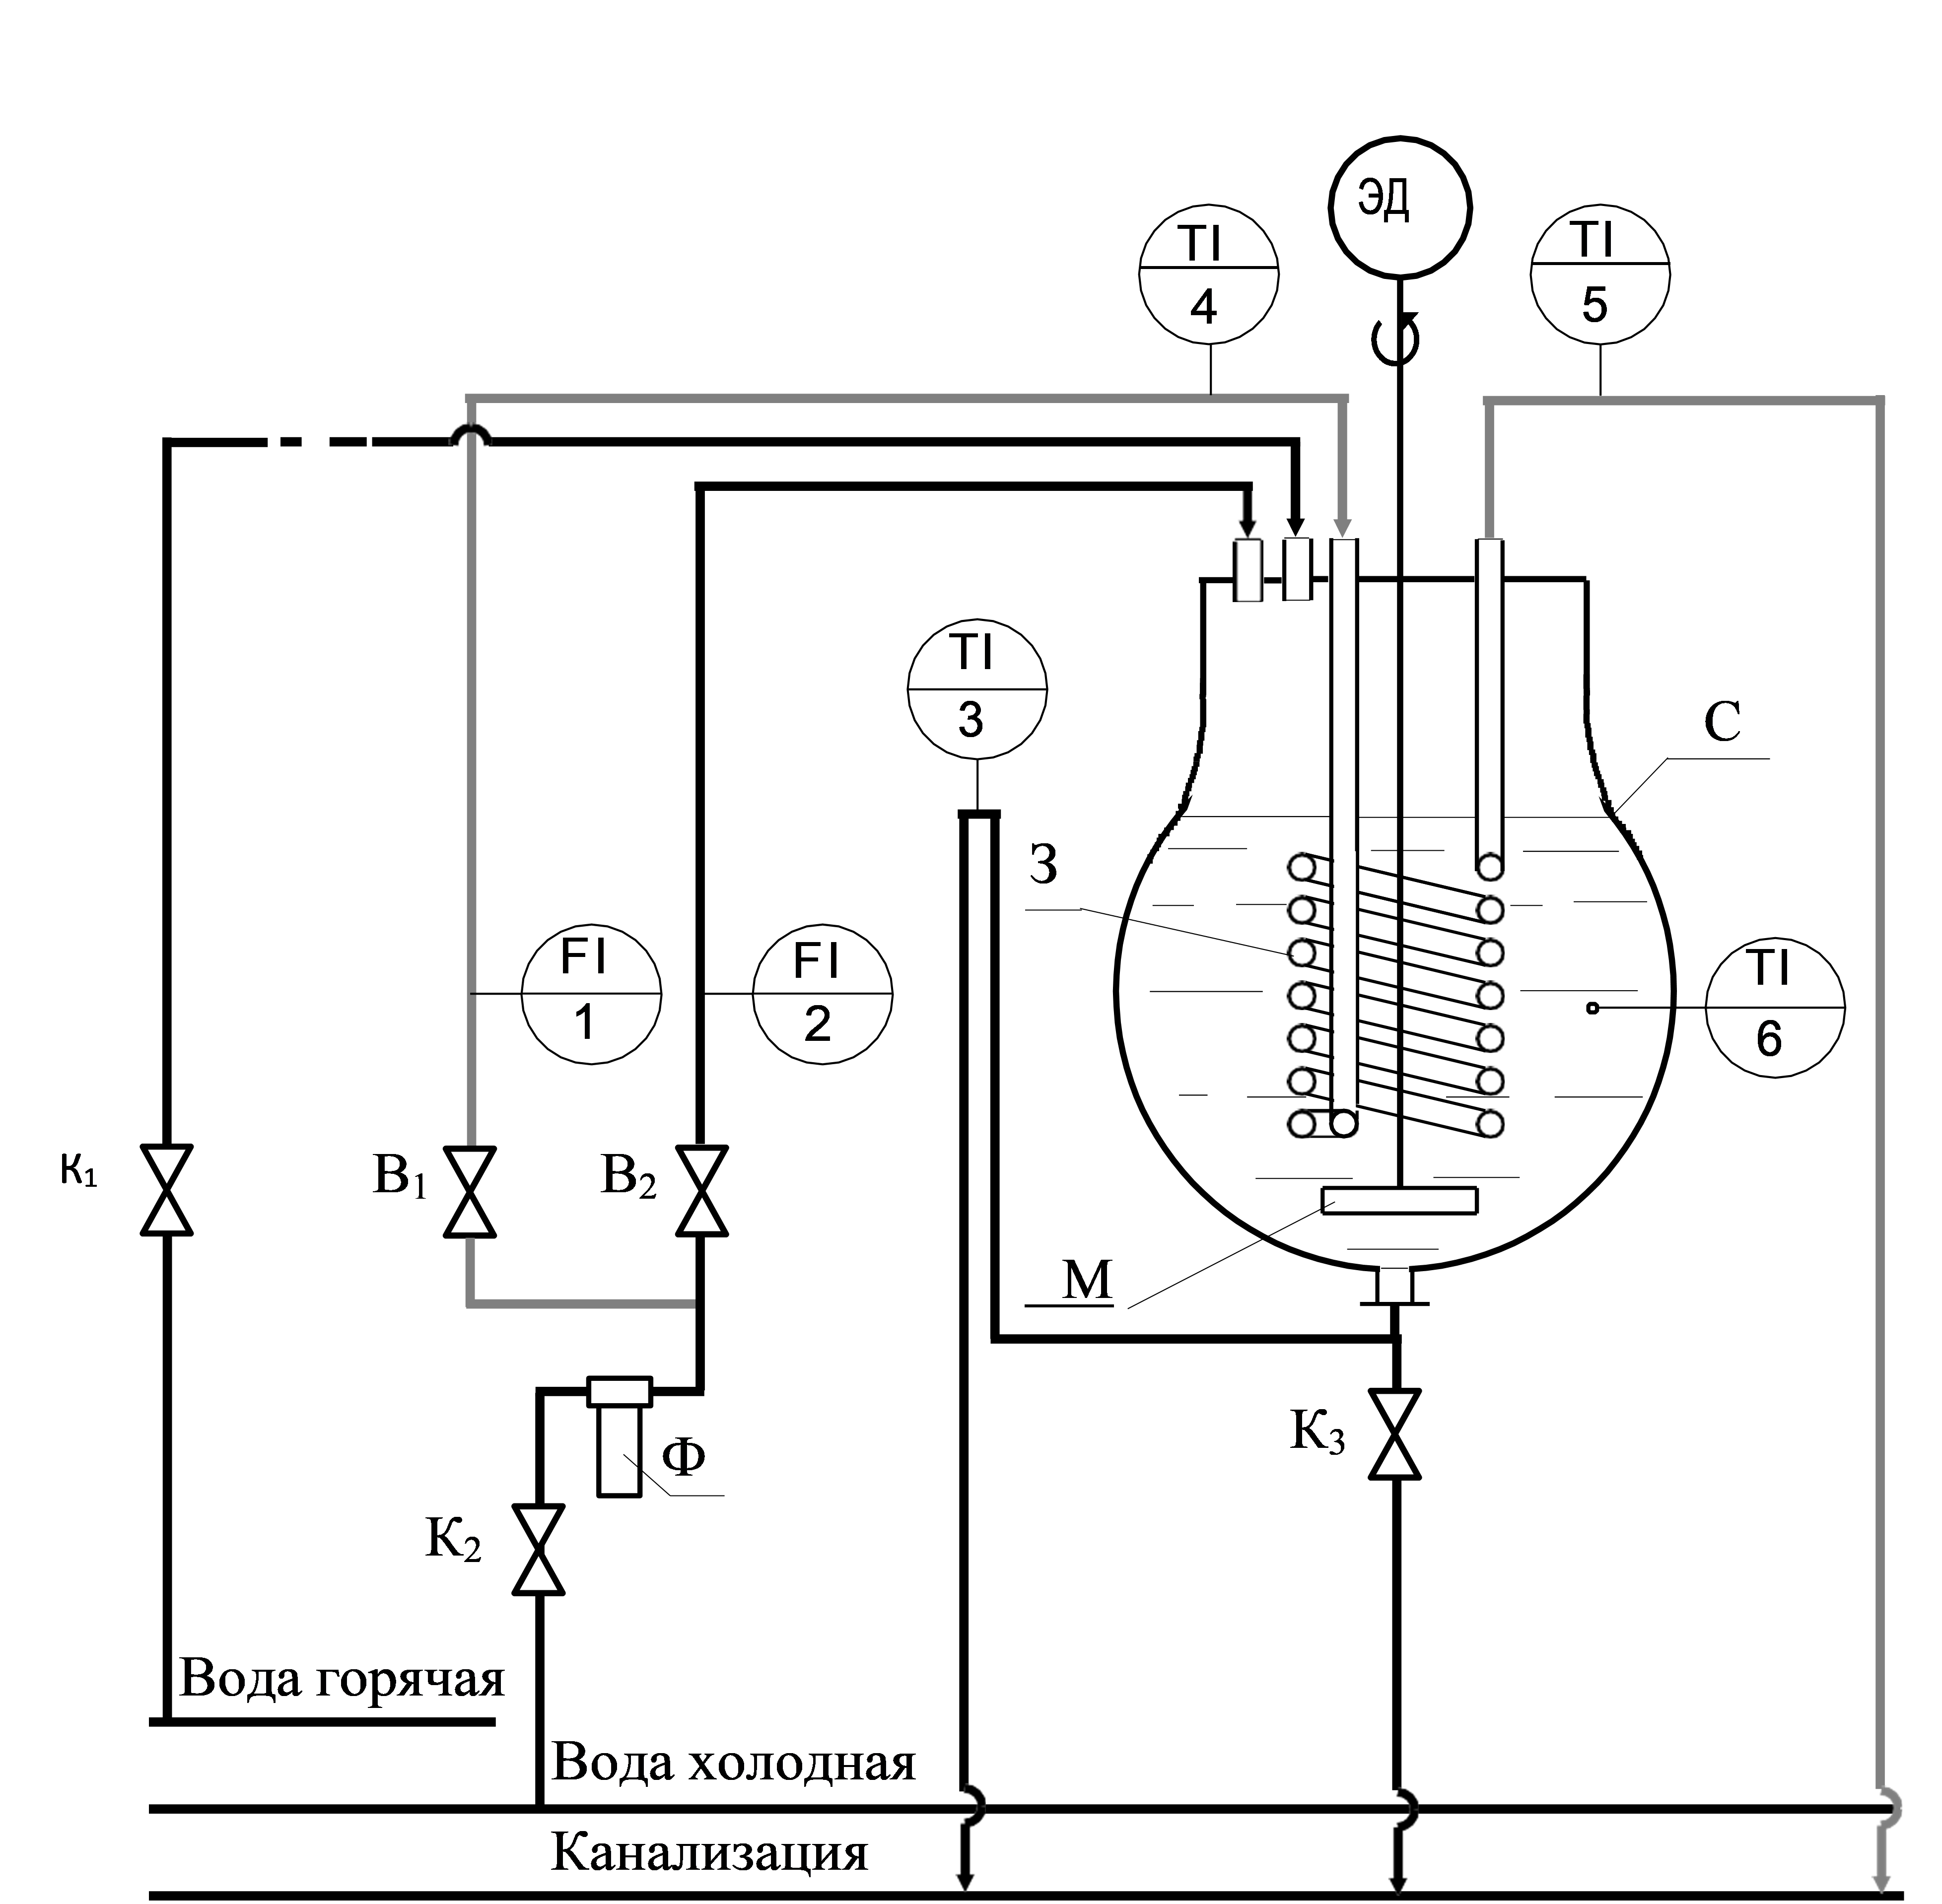
\includegraphics[width=0.7\textwidth]{img/schema.png}~
    \caption{Схема установки}
\end{figure}

Основным элементом установки является стеклянный реакционныйсосуд С грушевидной формы.\\

Благодаря специально организованному стоку воды через гидравлический затвор, объём жидкости в заполненном аппарате постоянен и равен $V_C = 24,57$ дм$^3$.
Средний диаметр заполненной части сосуда составляет $D_c = 0,292$ м.\\


Сосуд снабжён змеевиком З, изготовленным из стеклянной трубки размером {\diameter} 18,2 1,8 мм; диаметр витка змеевика $Dвит = 172,5$ мм. 
Площадь поверхности погруженной части змеевика, определённая по 
наружному размеру трубки $A = 0,405$ м$^2$. 
Боросиликатное стекло, из которого выполнен змеевик, имеет теплопроводность  ${\lambda}_{CT}$ = 1,14 Вт/(м K).\\

В змеевик может быть подана из водопровода холодная вода, протекающая через фильтр $\Phi$. Расход воды регулируется вентилем $В_1$ и измеряется ротáметром (поз. 1), имеющим на поверхности трубки шкалу, отградуированную в «л/мин» («LPM»).\\

Аппарат снабжён стеклянной лопастной мешалкой М диаметром $d_{M} = 136$ мм, 
вращаемой электродвигателем ЭД. Частота вращения мешалки $n = 2c^{-1}$.

Лабораторная установка оборудована электронными термометрами
(поз. 4, 5), установленными соответственно на линии подачи холодной воды и на линии выхода воды из змеевика. Температура в объёме сосуда измеряется ртутным термометром (поз. 6).


\newpage
\begin{center}
\subsection*{Обработка экспериментальных данных}
\end{center}
Экспериментальные данные (Таблица 1) используются для расчёта среднего значения коэффициента теплопередачи за период охлаждения и для расчёта
теоретического времени охлаждения жидкости при нестационарном теплообмене.\\


\begin{table}[!h]
\caption{Экспериментальные данных.}
\begin{center}
\begin{tabular}{|| c | c | c | c | c | c || c | c | c | c | c | c||} 
 \hline
 $i$ & $t_i$ & $T_{1,i}$ & $T_{2 in, i,}$ & $T_{2 out, i,}$ & 6,0 & $i$ & $t_i$ & $T_{1,i}$ & $T_{2 in, i,}$ & $T_{2 out, i,}$ & 6,0\\ [0.5ex] 
 \hline\hline
 0 & 0 & 13,5 & 25,2 & 50,8 & 44,9 & 20 & 10 & 6,3 & 28,1 & 50,9 & 43,5\\ 
 \hline
 1 & 0,5 & 11,6 & 33,8 & 50,8 & 46,1 & 21 & 10,5 & 6,3 & 28,1 & 51,1 & 42,8\\
 \hline
 2 & 1 & 8,2 & 33,6 & 51,1 & 46,6 & 22 & 11 & 6,3 & 28,0 & 51,1 & 43,1\\
 \hline
 3 & 1,5 & 7,1 & 29,7 & 51,1 & 46,2 & 23 & 11,5 & 6,3 & 27,9 & 51,2 & 42,8\\
 \hline
 4 & 2 & 6,5 & 27,9 & 51,3 & 45,5 & 24 & 12 & 6,3 & 27,7 & 51,2 & 42,6\\ 
 \hline
 5 & 2,5 & 6,5 & 27,3 & 51,3 & 44,9 & 25 & 12,5 & 6,3 & 27,6 & 51,3 & 42,3\\
 \hline
 6 & 3 & 6,4 & 26,7 & 51,5 & 43,9 & 26 & 13 & 6,4 & 27,4 & 51,3 & 42,1\\
 \hline
 7 & 3,5 & 6,3 & 26,5 & 51,1 & 43,9 & 27 & 13,5 & 6,4 & 27,2 & 51,3 & 41,9\\
 \hline
 8 & 4 & 6,2 & 26,3 & 50,7 & 43,4 & 28 & 14 & 6,4 & 27,1 & 51,2 & 41,8\\
 \hline
 9 & 4,5 & 6,2 & 26,0 & 50,6 & 43,1 & 29 & 14,5 & 6,4 & 27,0 & 51,1 & 41,6\\
 \hline
 10 & 5 & 6,1 & 25,9 & 50,5 & 42,7 & 30 & 15 & 6,4 & 26,8 & 51,1 & 41,4\\
 \hline
 11 & 5,5 & 6,2 & 25,8 & 50,7 & 42,4 & 31 & 15,5 & 6,3 & 26,7 & 51,0 & 41,3\\
 \hline
 12 & 6 & 6,2 & 25,7 & 50,6 & 42,1 & 32 & 16 & 6,3 & 26,6 & 51,0 & 41,1\\
 \hline
 13 & 6,5 & 6,2 & 25,6 & 50,8 & 41,9 & 33 & 16,5 & 6,3 & 26,6 & 51,0 & 41,0\\
 \hline
 14 & 7 & 6,2 & 25,6 & 50,6 & 41,7 & 34 & 17 & 6,2 & 26,5 & 51,2 & 40,9\\
 \hline
  15 & 7,5 & 6,2 & 25,5 & 50,8 & 41,4 & 35 & 17,5 & 6,3 & 26,5 & 51,2 & 40,8\\
 \hline
  16 & 8 & 6,3 & 25,4 & 50,7 & 41,3 & 36 & 18 & 6,2 & 26,4 & 51,1 & 40,7\\  
 \hline
  17 & 8,5 & 6,2 & 25,7 & 50,8 & 42,4 & 37 & 18,5 & 6,3 & 26,3 & 51,0 & 40,6\\  
 \hline
  89 & 9 & 6,3 & 27,4 & 50,7 & 43,4 & 38 & 19 & 6,3 & 26,3 & 51,0 & 40,6\\  
 \hline
  19 & 9,5 & 6,3 & 28,0 & 50,8 & 43,6 & 39 & 19,5 & 6,3 & 26,1 & 51,1 & 40,5\\ 
 \hline
  20 & 10 & 6,3 & 28,1 & 50,9 & 43,5 & 40 & 20 & 6,3 & 26,1 & 51,0 & 4,0\\\hline
\end{tabular}
\end{center}
\end{table}

\begin{table}[htbp]
\caption{Средние температуры за период охлаждения}
\begin{center}
\begin{tabular}{| c | c | c | c |}
 \hline
$T_{1,i}$ & $T_{2 in, i,}$ & $T_{2 out, i,}$ & 6,0 \\
 \hline
6,7 & 27,1 & 51,0 & 41,7 \\
  \hline
\end{tabular}
\end{center}
\end{table}

\begin{flushleft}
Выполнить следующие расчеты.
\end{flushleft}

\begin{center}
\subsection*{Анализ результатов работы}
\end{center}
 

\newpage
\begin{center}
\subsection*{Заключение}
\end{center}




\end{document}
%\usepackage[english,russian]{babel}